\documentclass[12pt]{article}
\usepackage{graphicx}
\usepackage{amsmath}
\usepackage{booktabs}
\usepackage{geometry}
\usepackage{hyperref}
\usepackage{subcaption} 
\usepackage{titlesec}
\usepackage{float}
\usepackage{svg}

\titlespacing*{\section}{0pt}{8pt}{5pt} % Section: {left}{before}{after}
\titlespacing*{\subsection}{0pt}{8pt}{4pt} % Subsection: {left}{before}{after}
\titlespacing*{\subsubsection}{0pt}{6pt}{3pt} % Subsubsection: {left}{before}{after}

\geometry{a4paper, margin=0.6in}

\begin{document}

\begin{titlepage}
    \centering
    \vspace{-2cm}
    \includesvg[width=0.6\textwidth]{birzeit-logo.svg}
    \vspace{1.5cm}


    {\Large Faculty of Engineering and Technology\\}
    {\Large Department of Electrical and Computer Engineering\\}
    \vspace{1cm}
    {\Large\bfseries \textbf{Computer Vision - ENCS5343}\\}


     \vspace{1.5cm}
    \rule{\textwidth}{0.4mm}\\
    \vspace{0.5cm}



    {\LARGE\bfseries
    Arabic Handwritten Text Identification Using Local Feature Extraction Techniques
     \\}
    \vspace{0.5cm}
    \rule{\textwidth}{0.4mm}\\
    
    \vspace{1.5cm}

    {\textbf{Prepared by:}\\ \vspace{0.5cm}}
    
    {\textbf{Mohammed Abed Alkareem - 1210708}\\}

    \vfill
    {\textbf{Supervisor:}\\ \vspace{0.5cm}}
    {\textbf{ Dr.Aziz Qaroush}}
    \vfill


    
    {\Large \text {Birzeit University}\\ \vspace{0.5cm}}

    {\Large \today}
\end{titlepage}

\section*{1. Objective}
The objective of this report is to evaluate and compare the performance of two local feature extraction techniques, SIFT (Scale-Invariant Feature Transform) and ORB (Oriented FAST and Rotated BRIEF), for identifying Arabic handwritten text. The focus is on assessing their accuracy, efficiency, and robustness across a variety of transformations and conditions.

\section*{2. Introduction}
Feature extraction is a crucial step in computer vision tasks. It enables systems to identify and differentiate patterns effectively. SIFT and ORB are popular local feature extraction techniques, each offering unique advantages. This report evaluates their performance on the AHAWP dataset, a benchmark dataset for handwritten Arabic text. The study aims to assess:
\begin{itemize}
    \item The quality of features extracted by each algorithm.
    \item Their robustness to transformations like noise, rotation, scale, and illumination changes.
    \item Their computational efficiency and generalization capabilities.
\end{itemize}
\section*{3. Dataset}

The AHAWP dataset consists of \textbf{8144 grayscale images} of \textbf{10 unique Arabic words}, handwritten by \textbf{82 individuals}. The dataset was divided into \textbf{60\% training} (\textbf{4886 images}), \textbf{20\% validation} (\textbf{1629 images}), and \textbf{20\% testing} (\textbf{1629 images}).

Preprocessing steps included the conversion of all images to grayscale for uniformity, augmentation of the test data with transformations such as Gaussian noise, rotation, scaling, and illumination changes to evaluate robustness, and the assignment of labels corresponding to the handwritten Arabic word represented in each image.

\section*{4. Methodology}

\subsection*{4.1 Feature Extraction}
\begin{itemize}
    \item \textbf{SIFT:} Extracts 128-dimensional descriptors for each key point, ensuring robustness to scale and rotation changes.
    \item \textbf{ORB:} Uses binary 32-dimensional descriptors for computational efficiency.
\end{itemize}

\subsection*{4.2 Feature Vector Formation}
\begin{itemize}
    \item Visual Bag of Words (vBoW) representation was constructed using KMeans clustering.
    \item TF-IDF was applied to generate fixed-length feature vectors, corresponding to the number of clusters (set as a hyperparameter).
    \item FAISS (Facebook AI Similarity Search) was employed for GPU-accelerated clustering.
\end{itemize}

\subsection*{4.3 Classification}
Logistic Regression was used to classify the feature vectors. Classifiers were trained on the training set and evaluated on the validation set.

\subsection*{4.4 Robustness Testing}
The test set was augmented with:
\begin{itemize}
    \item Gaussian Noise,
    \item Random Rotation (up to $\pm 30^\circ$),
    \item Scaling (0.5x to 1.5x),
    \item Illumination Changes (random contrast and brightness adjustments).
\end{itemize}

\begin{figure}[h!]
    \centering
    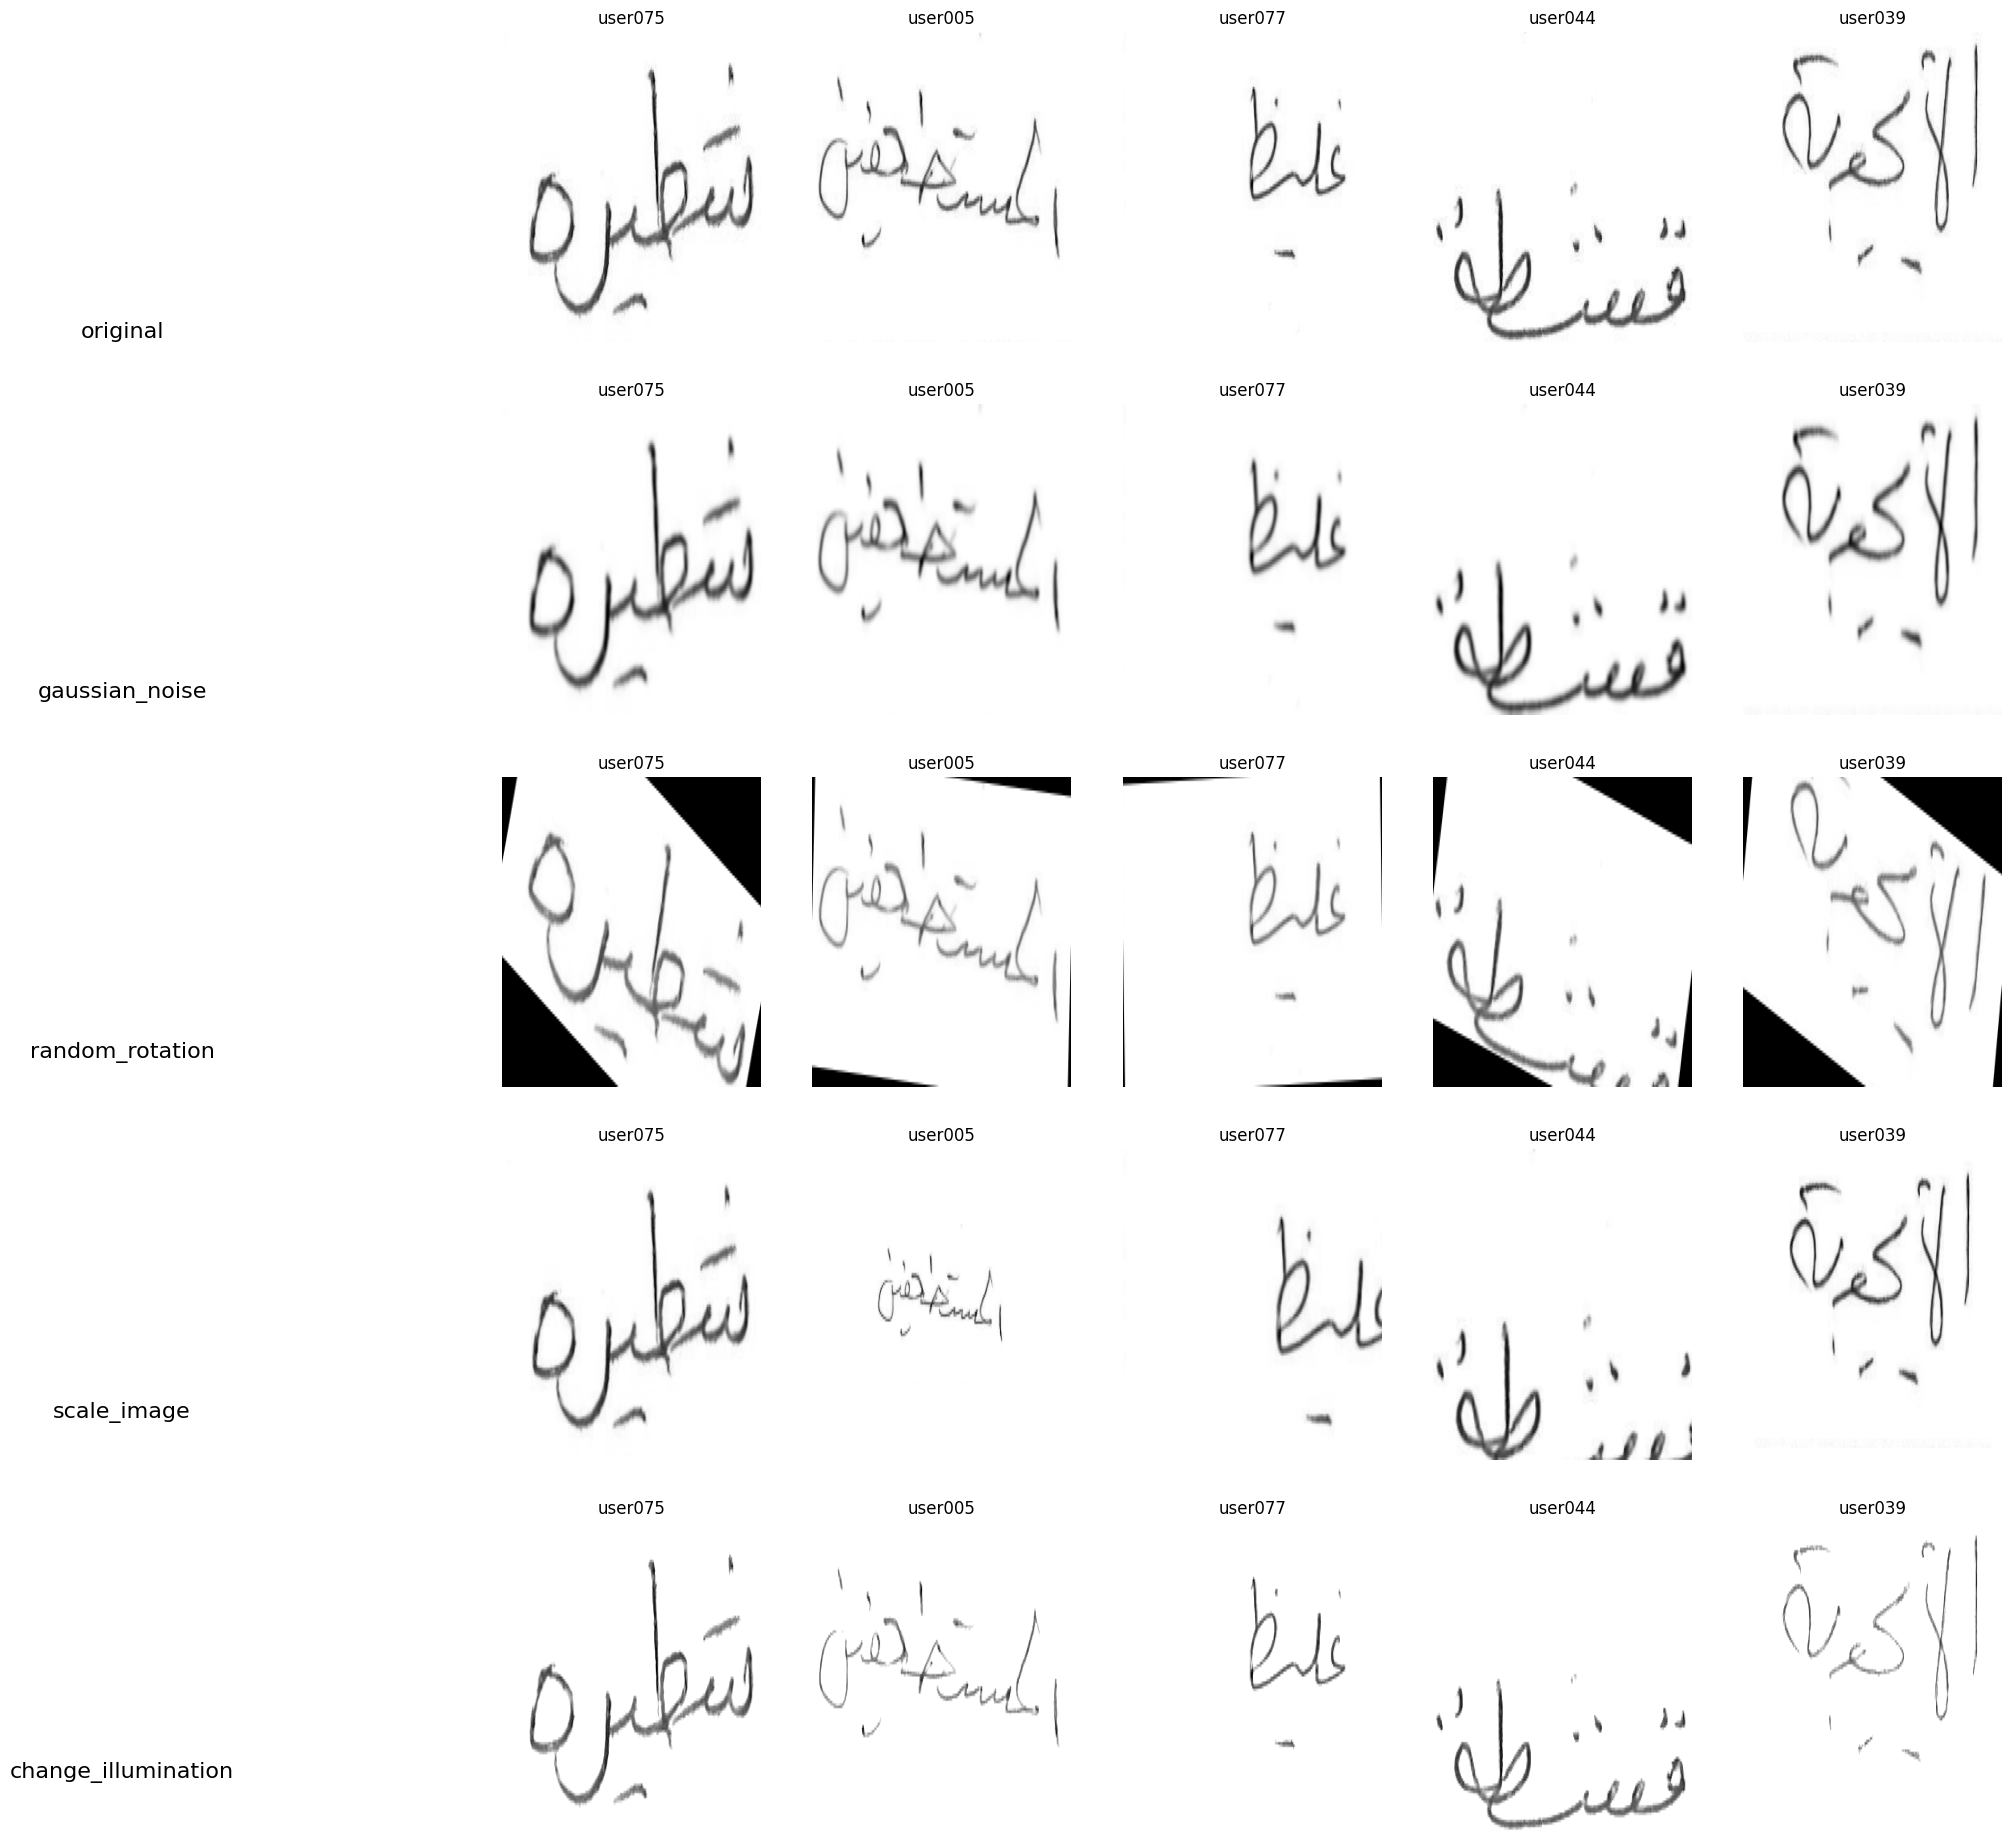
\includegraphics[width=0.5\textwidth]{figures/augmented.png} % Replace with your file path
    \caption{Augmented Datasets}
    \label{fig:robustness_chart}
\end{figure}

\section*{5. Metrics for Comparison}
The following metrics were used:
\begin{itemize}
    \item \textbf{Accuracy:} Percentage of correctly classified test cases.
    \item \textbf{Efficiency:} Execution time for feature extraction, clustering, and feature vector formation.
    \item \textbf{Robustness:} Performance on augmented test sets.
    \item \textbf{Number of Key Points:} Average number of key points detected per image.
\end{itemize}

\section*{6. Results and Analysis}

\subsection*{6.1 Efficiency Comparison}
\begin{table}[H]
\centering
\begin{tabular}{@{}lccc@{}}
\toprule
\textbf{Metric}                            & \textbf{SIFT}   & \textbf{ORB}    \\ \midrule
Number of Processed Images                 & 8144            & 8144            \\
Average Key Points per Image               & 90.99           & 175.94          \\
Average Feature Extraction Time (s/image)  & 0.01072         & 0.00135         \\
Clustering Time (1000 Clusters) (s)        & 2.54            & 0.95            \\
Feature Vector Formation Time (s)          & 2.79            & 5.64            \\ \bottomrule
\end{tabular}
\caption{Efficiency comparison of SIFT and ORB.}
\label{tab:efficiency_comparison}
\end{table}

\textbf{} 
The efficiency results highlight a trade-off between speed and descriptor quality for SIFT and ORB. ORB processes features faster, with an average extraction time of \textbf{0.00135 seconds per image} compared to SIFT's \textbf{0.01072 seconds}, and achieves faster clustering (\textbf{0.95 seconds versus 2.54 seconds)}. This efficiency stems from ORB's binary descriptors and higher average key point detection (\textbf{175.94 vs. 90.99}). However, the feature vector formation time for ORB \textbf{(5.64 seconds)} is longer than SIFT's \textbf{(2.79 seconds)} due to its higher key point count. 

\subsection*{6.2 Clustering and Accuracy Analysis}

\begin{table}[H]
\centering
\begin{tabular}{@{}lccc@{}}
\toprule
\textbf{Algorithm} & \textbf{Number of Clusters} & \textbf{Training Accuracy (\%)} & \textbf{Validation Accuracy (\%)} \\ \midrule
SIFT               & 100                         & 19.00                           & 11.00                             \\
SIFT               & 1300                        & 60.00                           & 21.00                             \\
SIFT               & 4300                        & 84.00                           & 24.00                             \\ \midrule
ORB                & 100                         & 10.00                           & 6.00                              \\
ORB                & 1300                        & 30.00                           & 9.00                              \\
ORB                & 4300                        & 47.00                           & 9.00                              \\ \bottomrule
\end{tabular}
\caption{Accuracy comparison for different cluster sizes.}
\label{tab:accuracy_comparison}
\end{table}

\textbf{} The results indicate evidence of \textit{overfitting} as the number of clusters increases, particularly for \textbf{SIFT}. While SIFT’s training accuracy improves significantly from \textbf{19.00\%} at 100 clusters to \textbf{84.00\%} at 4300 clusters, the corresponding validation accuracy increases more modestly, from \textbf{11.00\%} to \textbf{24.00\%}. This widening gap suggests that the model may be memorizing training data rather than generalizing effectively to unseen validation data. For \textbf{ORB}, overfitting is less pronounced, but its validation accuracy stagnates at \textbf{9.00\%}, even as training accuracy rises to \textbf{47.00\%} at 4300 clusters. This indicates that ORB's descriptors are not robust enough to capitalize on the additional clusters, resulting in limited generalization capacity. These results emphasize the need to balance cluster complexity to avoid overfitting while maintaining generalization.
\begin{figure}[H]
    \centering
    \begin{subfigure}[b]{0.3\textwidth} % Reduced width to 30% of text width
        \centering
        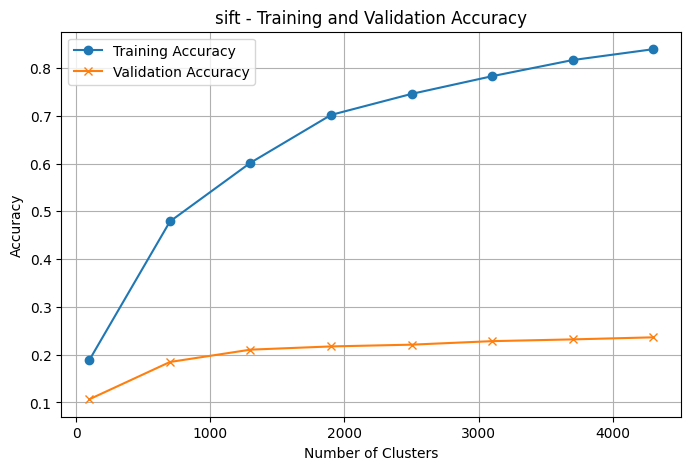
\includegraphics[width=\textwidth]{figures/sift.png} % Replace with your file path
        \caption{Accuracy of SIFT.}
        \label{fig:efficiency_chart}
    \end{subfigure}
    \hspace{0.01\textwidth} % Add small space between the subfigures
    \begin{subfigure}[b]{0.3\textwidth} % Reduced width to 30% of text width
        \centering
        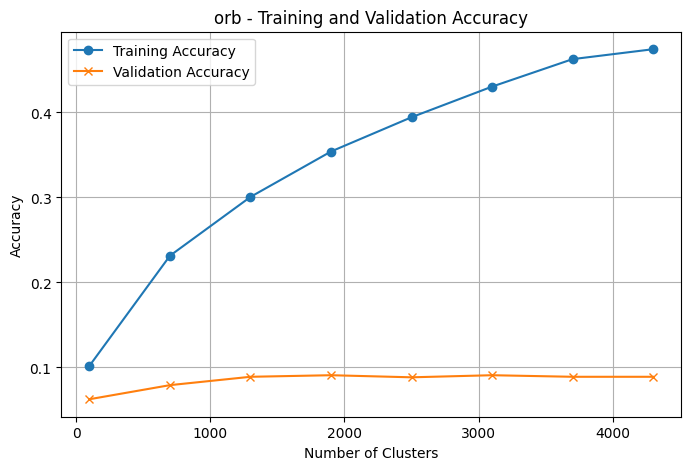
\includegraphics[width=\textwidth]{figures/orb.png} % Replace with your file path
        \caption{Accuracy of ORB.}
        \label{fig:accuracy_vs_clusters}
    \end{subfigure}
    \caption{Comparison of SIFT and ORB for training and validation accuracy.}
    \label{fig:side_by_side}
\end{figure}


\subsection*{6.3 Robustness Evaluation}
\begin{table}[h!]
\centering
\begin{tabular}{@{}lcccccc@{}}
\toprule
\textbf{Algorithm} & \textbf{Test Set}         & \textbf{Original} & \textbf{Gaussian Noise} & \textbf{Rotation} & \textbf{Scale} & \textbf{Illumination} \\ \midrule
SIFT               & Accuracy (\%)            & 21.00             & 10.00                   & 18.00             & 16.00          & 17.00                 \\
ORB                & Accuracy (\%)            & 8.00              & 8.00                    & 9.00              & 6.00           & 5.00                  \\ \bottomrule
\end{tabular}
\caption{Robustness comparison of SIFT and ORB.}
\label{tab:robustness_comparison}
\end{table}

\textbf{} The robustness results highlight that SIFT outperforms ORB across all test conditions. On the original test set, SIFT achieves significantly higher accuracy (\textbf{21.00\%}) compared to ORB (\textbf{8.00\%}). Under transformations such as Gaussian noise, rotation, scaling, and illumination changes, SIFT demonstrates superior resilience, achieving accuracies of \textbf{10.00\%}, \textbf{18.00\%}, \textbf{16.00\%}, and \textbf{17.00\%}, respectively. In contrast, ORB's performance remains consistently low, with accuracies peaking at \textbf{9.00\%} for rotation and dropping as low as \textbf{5.00\%} for illumination changes. These results underline SIFT’s robustness and adaptability to real-world variability, whereas ORB is limited to controlled environments due to its less discriminative binary descriptors.


\begin{figure}[h!]
    \centering
    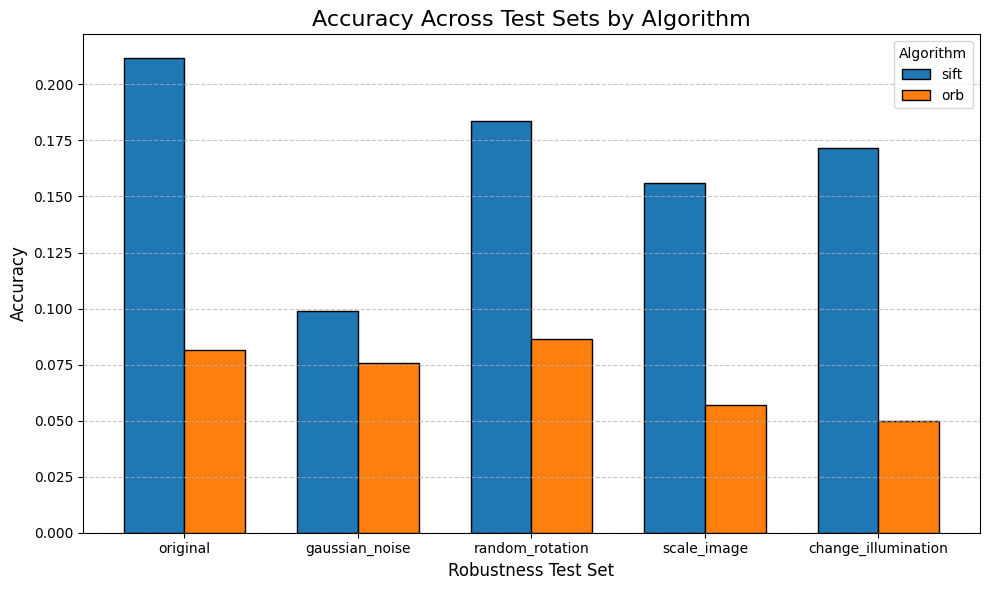
\includegraphics[width=0.5\textwidth]{figures/robust.png} % Replace with your file path
    \caption{Robustness comparison of SIFT and ORB across transformations.}
    \label{fig:robustness_chart}
\end{figure}

\section*{7. Conclusion}
This study highlights the strengths and limitations of SIFT and ORB for handwritten Arabic text identification:
\begin{itemize}
    \item \textbf{SIFT:} Superior robustness, accuracy, and generalization make it suitable for high-precision tasks. Its ability to handle transformations such as rotation and illumination changes demonstrates its effectiveness for challenging scenarios.
    \item \textbf{ORB:} Faster processing and computational efficiency make it ideal for applications prioritizing speed. However, its limited descriptor quality reduces its effectiveness for complex or noisy data.
\end{itemize}

Future work could explore hybrid approaches that combine SIFT’s robustness with ORB’s efficiency. Additionally, integrating preprocessing techniques to handle noisy or distorted images could further improve overall performance.

\section*{8. References}
\begin{enumerate}
    \item Lowe, D. G. (2004). "Distinctive Image Features from Scale-Invariant Keypoints." \textit{International Journal of Computer Vision}.
    \item Rublee, E., et al. (2011). "ORB: An efficient alternative to SIFT or SURF." \textit{Proceedings of ICCV}.
    \item AHAWP Dataset. \url{https://data.mendeley.com/datasets/2h76672znt/1/files/9031138a-b812-433e-a704-8acb1707936e}.
    \item Johnson, J., et al. (2019). "Billion-scale similarity search with FAISS." \textit{IEEE Transactions on Big Data}.
\end{enumerate}

\end{document}
